\documentclass[12pt, a4paper]{article}
\usepackage[russian]{babel}
\usepackage[utf8]{inputenc}
\usepackage[T2A]{fontenc}
\usepackage{amsfonts}
\usepackage{amsmath}
\usepackage[
left 	= 	30	mm,
right 	=	15	mm,
top 	=	20	mm,
bottom 	=	20	mm,
]{geometry}

\usepackage{indentfirst} % Красная строка

\setlength{\parindent}{1.25 cm}

\usepackage[toc,page]{appendix}

\renewcommand{\baselinestretch}{1.5}

\usepackage{titlesec}

\titleformat{\section}
{\normalfont\fontsize{14}{14}\bfseries}{\thesection}{1em}{}

\titleformat{\subsection}
{\normalfont\fontsize{14}{14}\bfseries}{\thesubsection}{1em}{}

\usepackage[intoc]{nomencl}
\renewcommand{\nomname}{Обозначения и сокращения}
\makenomenclature

%%% Математика

% Шрифты для математики
\usepackage{amsmath}
\usepackage{amsfonts}
\usepackage{amssymb}
\usepackage{cancel}
\usepackage{mathrsfs}
\usepackage{mathtools}
\usepackage{upgreek}
\usepackage{xfrac}


%%% Иллюстрации
\usepackage{graphicx}
\usepackage{subcaption}
\usepackage{wrapfig}
\usepackage[export]{adjustbox}
%\graphicspath{{./img/}}

\makeatletter % список литературы
\def\@biblabel#1{#1. }
\makeatother

% Графики
\usepackage{pgfplots}
\pgfplotsset{compat=1.3}
\usepgfplotslibrary{patchplots}
%\usepackage{patchplots}
\pgfplotsset{	width	=	14	cm,
	x label style={
		font = {\small\sffamily},
		yshift = 1mm
	},
	tick label style={
		font = {\scriptsize},
	},
	y label style={
		font = {\small\sffamily},
		yshift = -1mm,
		at={(ticklabel cs:0.5)},
		%      					rotate=90,
		anchor=near ticklabel
	},
	every tick/.style	=	{
		black, 
		line width 	= 	.5	pt
	},
	axis line style 	= 	{
		line width 	= 	.5	pt
	},
	grid style	=	{
		gray,
		dotted
	},
	minor x tick num = 1,
	minor y tick num = 1,
	no markers,
	grid = major,
	every axis/.append style	=	{
		line width	=	.7	pt
	}
}

%Подписи
\usepackage		[margin		= 10	pt,
%					font		= footnotesize, 
%labelfont	= bf, 
labelsep	= endash, 
%labelfont	= bf,
%					textfont	= sl,
margin		= 0 	pt,  
aboveskip 	= 4		pt, 
belowskip 	= -6	pt,
figurename= Рисунок] {caption}
\usepackage		[margin		= 10	pt,
font		= footnotesize, 
labelfont	= bf, 
labelsep	= endash, 
labelfont	= bf,
textfont	= sl,
margin		= 0 	pt,  
aboveskip 	= 4		pt, 
belowskip 	= 6	pt]	{subcaption}

\makeatletter
%\newcounter{figure}[section]
%\newcounter{table}[section]
\renewcommand{\thefigure}{\thesection.\@arabic\c@figure}
\renewcommand{\thetable}{\thesection.\@arabic\c@table}
\makeatother


%%% Insert pdf pages
\usepackage[final]{pdfpages}


%%% Color highlight
\usepackage{xcolor}

% Ссылки внутри текста
\usepackage{hyperref}

% Настройка листингов
\usepackage{listings}
\lstset{
	language = sql,
	extendedchars=\true,
	keepspaces=true,
	basicstyle=\scriptsize\sffamily,
	showstringspaces=\false,
	numbers=left,
	stepnumber=1,
	numbersep=5pt,
	frame=single,
	tabsize=2,
	captionpos=t,
	breaklines=true,
	breakatwhitespace=false,
	escapeinside={\#*}{*)}
}

% Чтобы вместо : в подписях было -
\RequirePackage{caption}
\DeclareCaptionLabelSeparator{defffis}{ — }
\captionsetup{justification=centering,labelsep=defffis}

\usepackage{pgfplots}
\usepackage{pgfplotstable}
\pgfplotsset{compat=1.9}

\begin{document}
	
\includepdf[pages=1]{inc/title.pdf}
	
	%\tableofcontents
	%\newpage
	
	\section{Задание}
	Необходимо промоделировать работу прибора обслуживания, определить длину очереди, при которой не будет потерянных сообщений и вывести результат на экран. 

Закон генерации сообщений равномерный, обслуживание происходит согласно закону в соответствии с вариантом: \textbf{нормальный}.

Следует предусмотреть возможность построения обратной связи, указывая в процентах долю заявок, которые возвращаются назад в очередь. 

Реализовать двумя способами: событийный и пошаговый.
	%\newpage
	
	\section{Теоретическая часть}
	\subsection{Равномерное распределение}

Функция распределения имеет вид:
\begin{equation}
	F_X(x) = 
	\left\{\begin{array}{l}
		0, x < a, \\
		\frac{x - a}{b - a}, a \leq x < b, \\
		1, x \geq b.
	\end{array}\right.
\end{equation}

\subsection{Нормальное распределение}

Функция распределения имеет вид:
\begin{equation}
	F_X(x) = \frac{1}{\sigma \sqrt{2 \pi}} \int\limits_{-\infty}^x e^{-\dfrac{(x - \mu)^2}{2 \sigma^2}} \,dx
\end{equation}

Стандартным нормальным распределением называется нормальное распределение с математическим ожиданием $\mu = 0$ и стандартным отклонением $\sigma = 1$.

\subsection{Пошаговый принцип ($\Delta t$)}
Этот принцип заключается в последовательном анализе состояний всех блоков системы в момент $t + \Delta t$. При этом новое состояние блоков определяется в соответствии с их алгоритмическим описанием. 

Недостаток: значительные временные затраты на реализацию моделирования системы. А также при недостаточно малом $\Delta t$ отдельные события в системе могут быть пропущены, что может повлиять на адекватность результатов.

\subsection{Событийный принцип}
Состояние отдельных устройств изменяются в дискретные моменты времени, совпадающие с моментами времени поступления сообщений в систему, временем окончания обработки задачи и т.д.

При использовании событийного принципа состояние всех блоков системы анализируется лишь в момент проявления какого-либо события. Моменты наступления следующего события определяются минимальным значением из списка событий.


	\newpage
	
	\newpage
	\section{Код программы}
	В листинге \ref{code} представлены основные методы.

\begin{lstlisting}[label=code, caption = Основные методы]
func eventModel(_ generator: EvenDistribution, _ processor: NormalDistribution, _ totalTasks: Int = 0, _ repeat_percentage: Int = 0) -> Int {
    var processedTasks = 0
    var curQueueLen = 0
    var maxQueueLen = 0
    var events: [(Double, String)] = [(generator.generate(), "g")]
    var free = true
    var processFlag = false
    
    while processedTasks < totalTasks {
        let event = events.removeFirst()
        if event.1 == "g" {
            curQueueLen += 1
            if curQueueLen > maxQueueLen {
                maxQueueLen = curQueueLen
            }
            addEvent(&events, (event.0 + generator.generate(), "g"))
            
            if free {
                processFlag = true
            }
        } else if event.1 == "p" {
            processedTasks += 1
            
            if Int.random(in: 1...100) <= repeat_percentage {
                curQueueLen += 1
            }
            processFlag = true
        }
        
        if processFlag {
            if curQueueLen > 0 {
                curQueueLen -= 1
                addEvent(&events, (event.0 + processor.generate(), "p"))
                free = false
            } else {
                free = true
            }
            processFlag = false
        }
    }
    
    return maxQueueLen
}

func addEvent(_ events: inout [(Double, String)], _ newEvent: (Double, String)) {
    var i = 0
    
    while i < events.count && events[i].0 < newEvent.0 {
        i += 1
    }
    
    0 < i && i < events.count ? events.insert(newEvent, at: i - 1) : events.insert(newEvent, at: i)
}

func stepModel(_ generator: EvenDistribution, _ processor: NormalDistribution, _ totalTasks: Int, _ repeat_percentage: Int, _ step: Double) -> Int {
    var processedTasks = 0
    var tCurr: Double = step
    var tGen = generator.generate()
    var tGenPrev: Double = 0
    var tProc: Double = 0
    var curQueueLen = 0
    var maxQueueLen = 0
    var free = true
    
    while processedTasks < totalTasks {
        if tCurr > tGen {
            curQueueLen += 1
            
            if curQueueLen > maxQueueLen {
                maxQueueLen = curQueueLen
            }
            
            tGenPrev = tGen
            tGen += generator.generate()
        }
            
        if tCurr > tProc {
            if curQueueLen > 0 {
                let wasFree = free
                if free {
                    free = false
                } else {
                    processedTasks += 1
                    if Int.random(in: 1...100) <= repeat_percentage {
                        curQueueLen += 1
                    }
                }
                
                curQueueLen -= 1
                
                if wasFree {
                    tProc = tGenPrev + processor.generate()
                } else {
                    tProc += processor.generate()
                }
                
            } else {
                free = true
            }
        }
        tCurr += step
    }
            
    return maxQueueLen
}
\end{lstlisting}
	
	\section{Результаты работы программы}
	Интерфейс предполагает ввод всех необходимых параметров модели. Моделирование происходит до тех пор, пока не будет обработано 1\,000 сообщений. 

Также предоставляется возможность указания в процентах объема сообщений, которые возвращаются обратно в очередь.

На рисунках \ref{fig1:image} -- \ref{fig5:image} демонстрируются результаты работы.

\begin{figure}[h!]
	\begin{center}
		{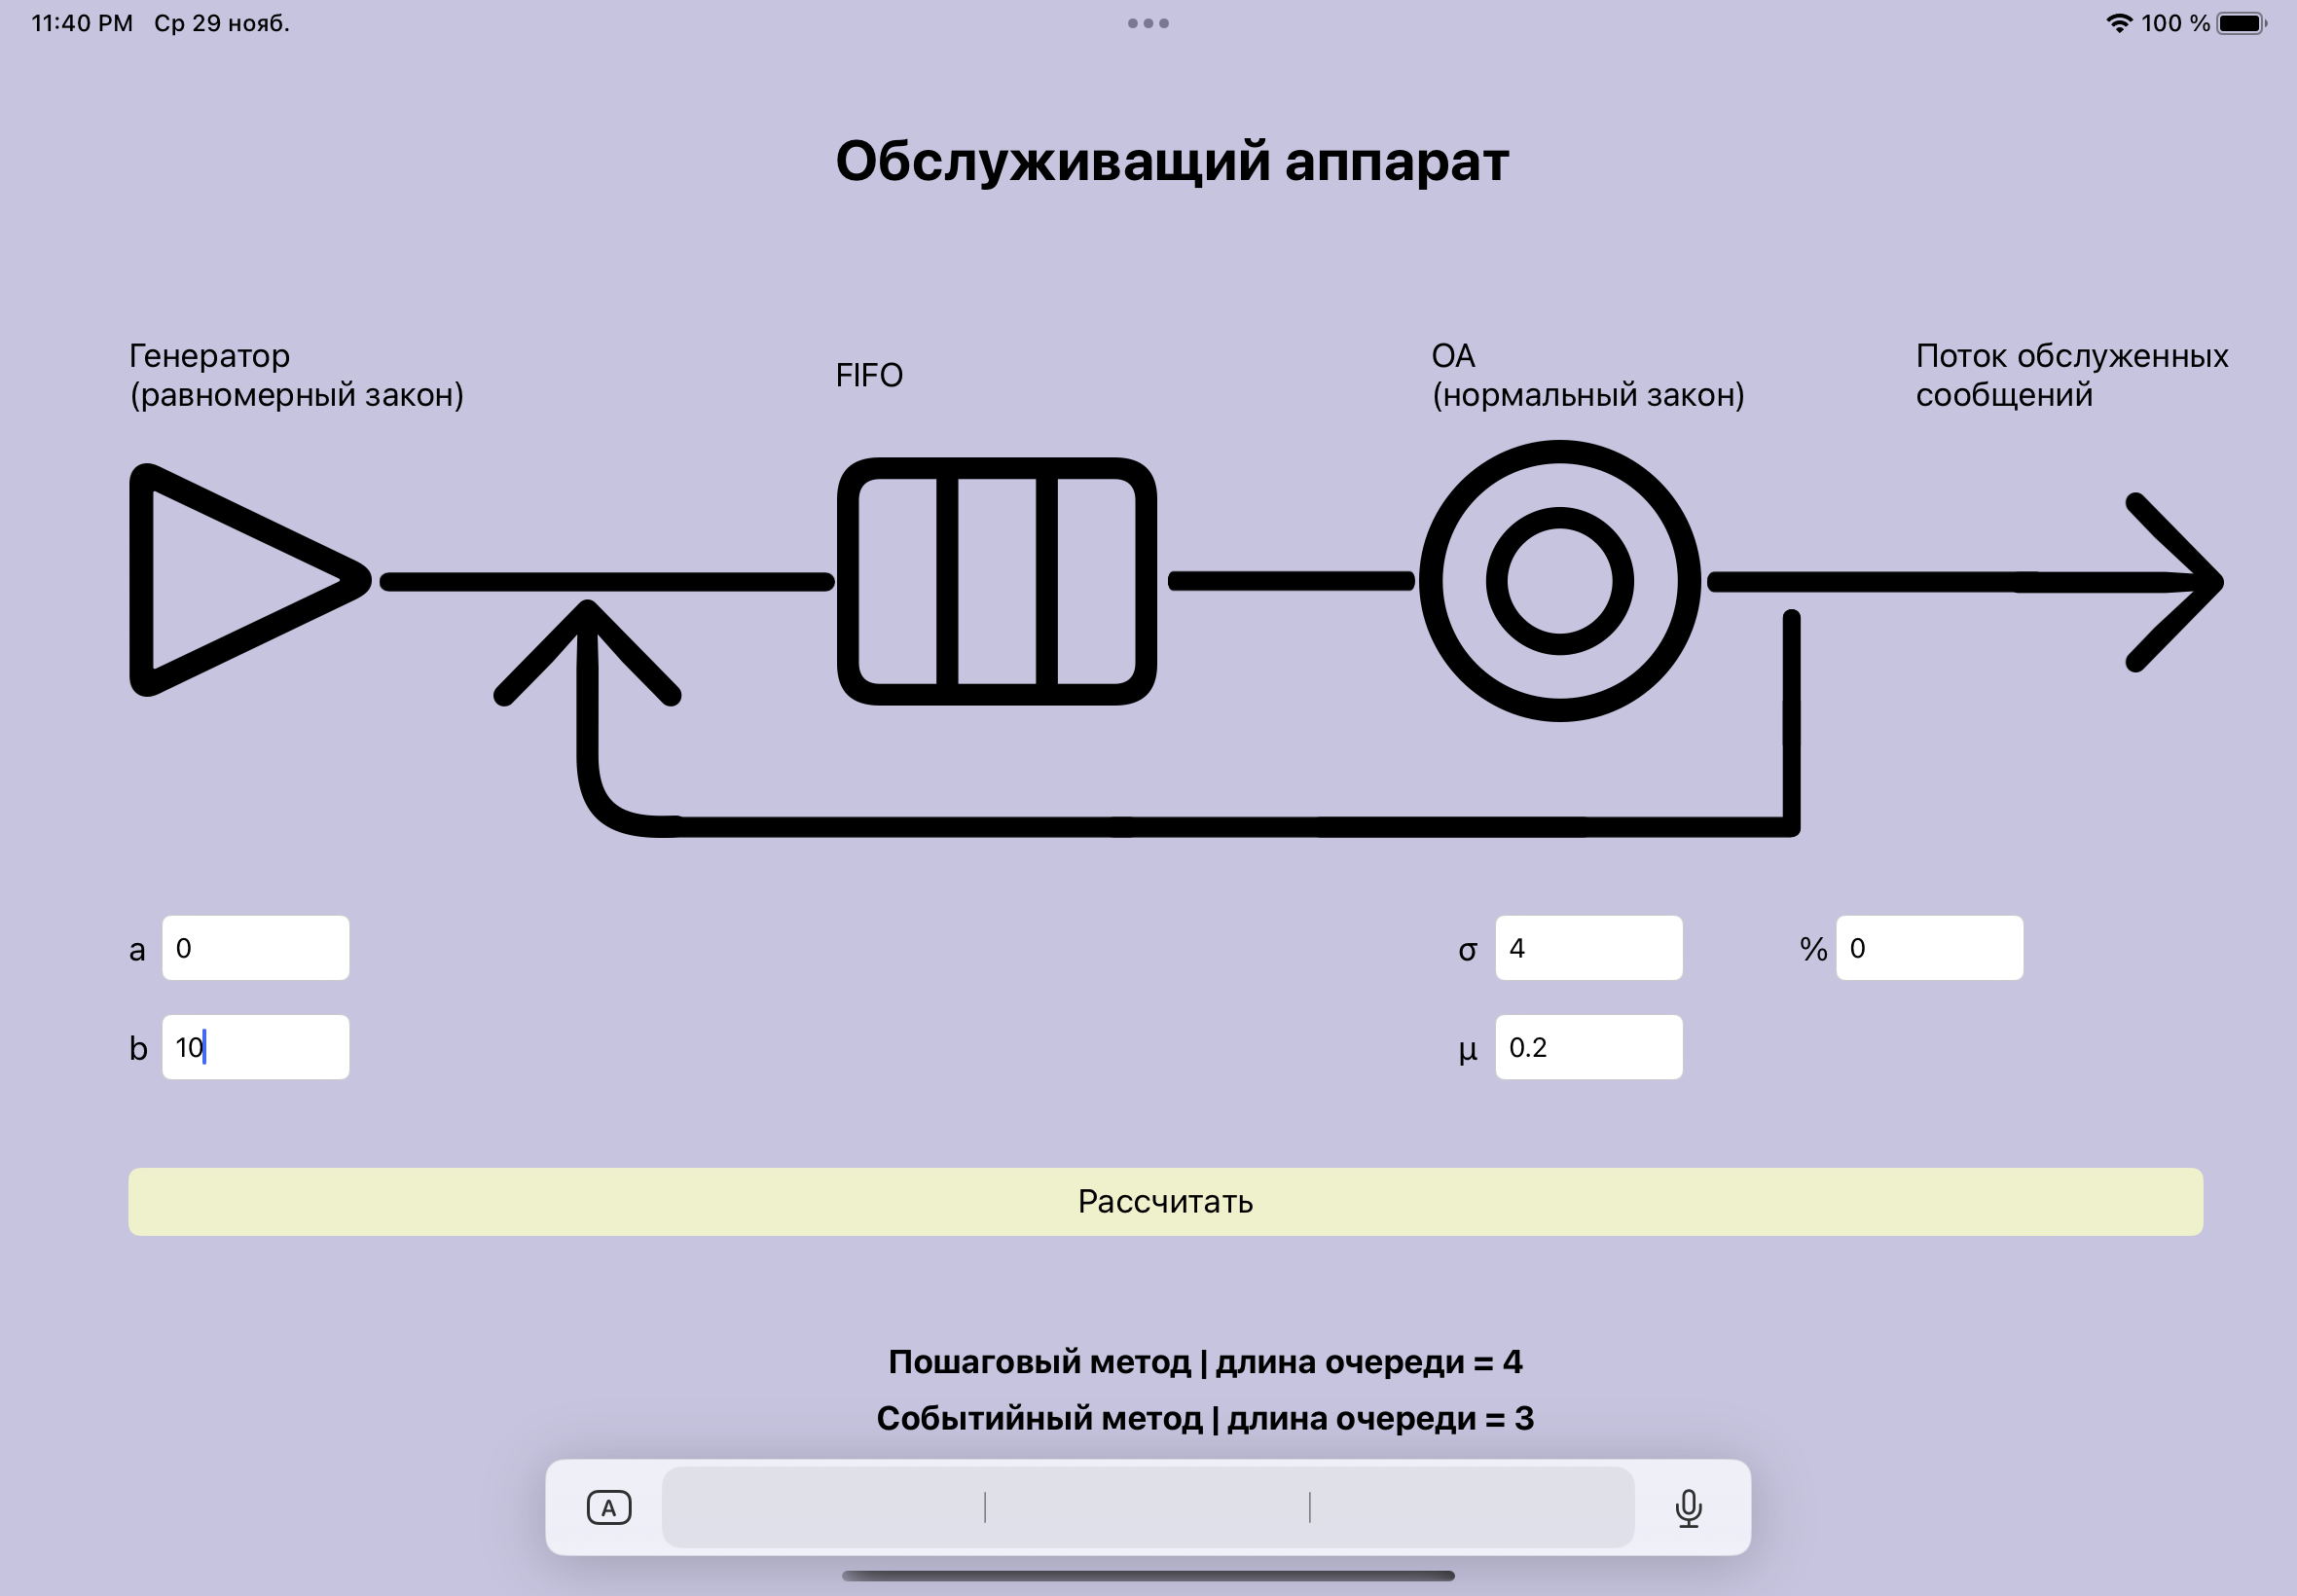
\includegraphics[scale = 0.15]{img/ex1.png}}
		\caption{Пример 1. Генератор и обслуживающий автомат работают с примерно одинаковой производительностью}
		\label{fig1:image}
	\end{center}
\end{figure}

\begin{figure}[h!]
	\begin{center}
		{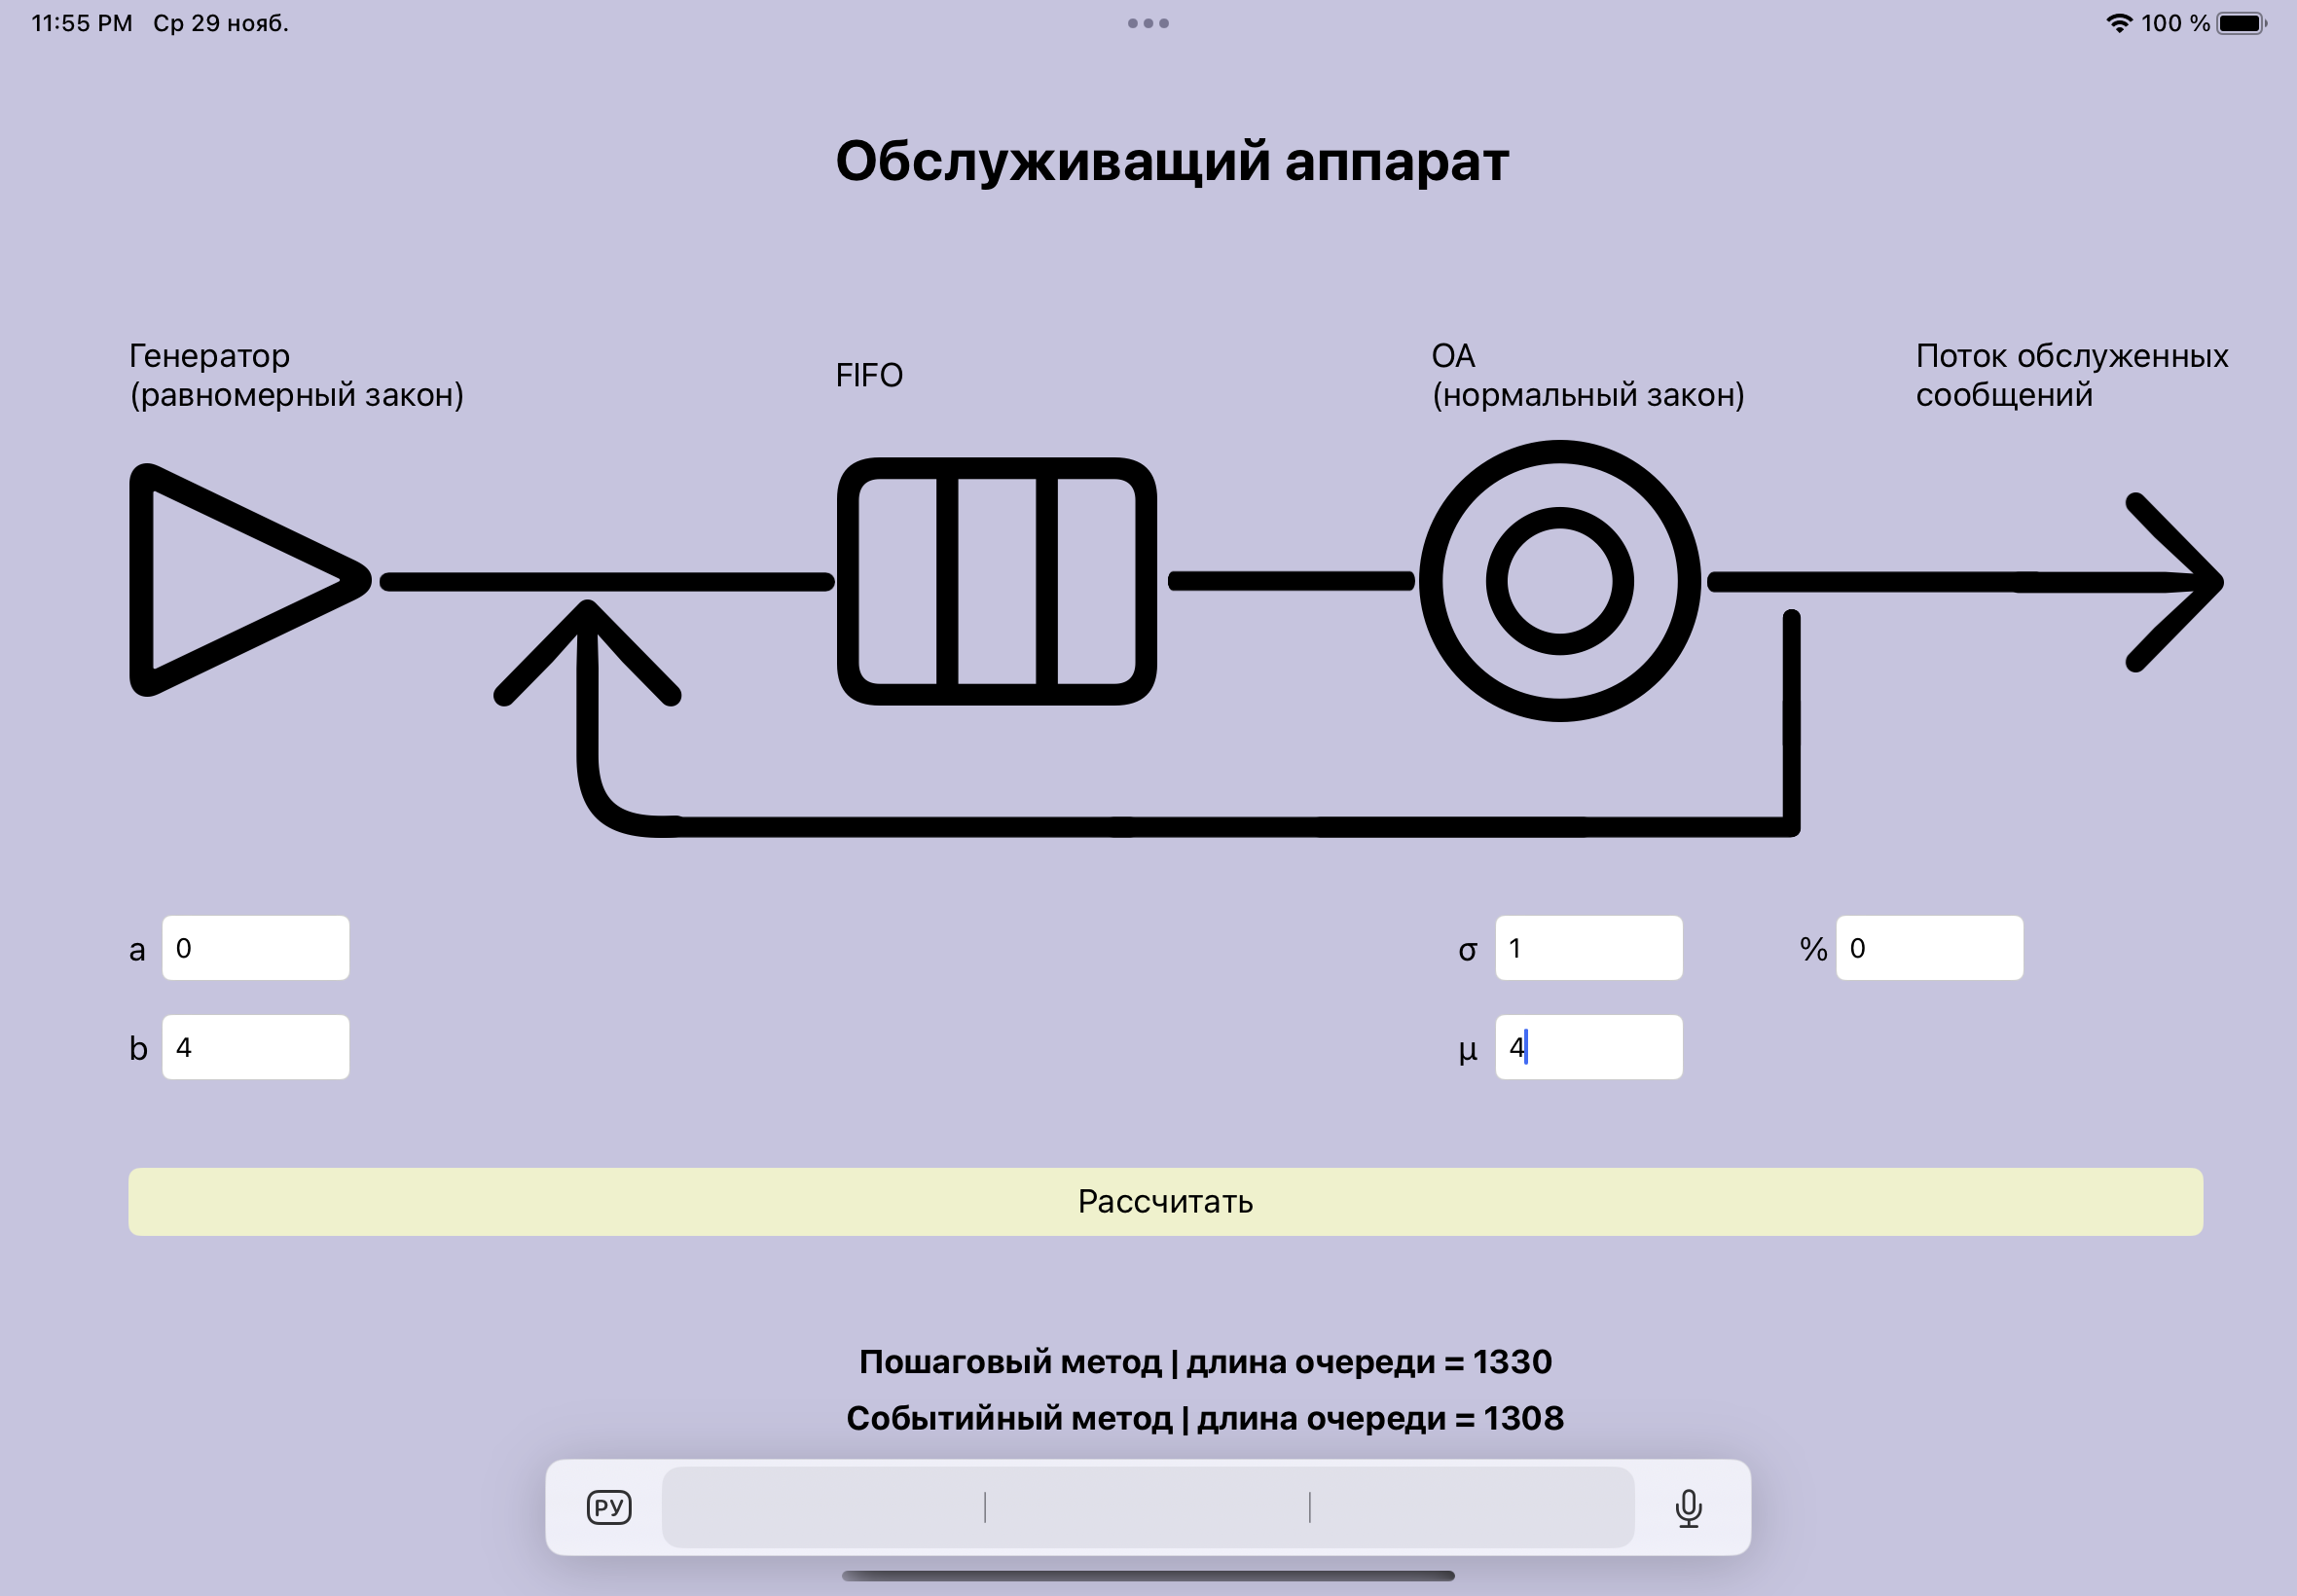
\includegraphics[scale = 0.15]{img/ex2.png}}
		\caption{Пример 2. Генератор создает сообщения интенсивнее, чем их обрабатывает автомат (при таких параметрах возникает переполнение)}
		\label{fig2:image}
	\end{center}
\end{figure}
\newpage

\begin{figure}[h!]
	\begin{center}
		{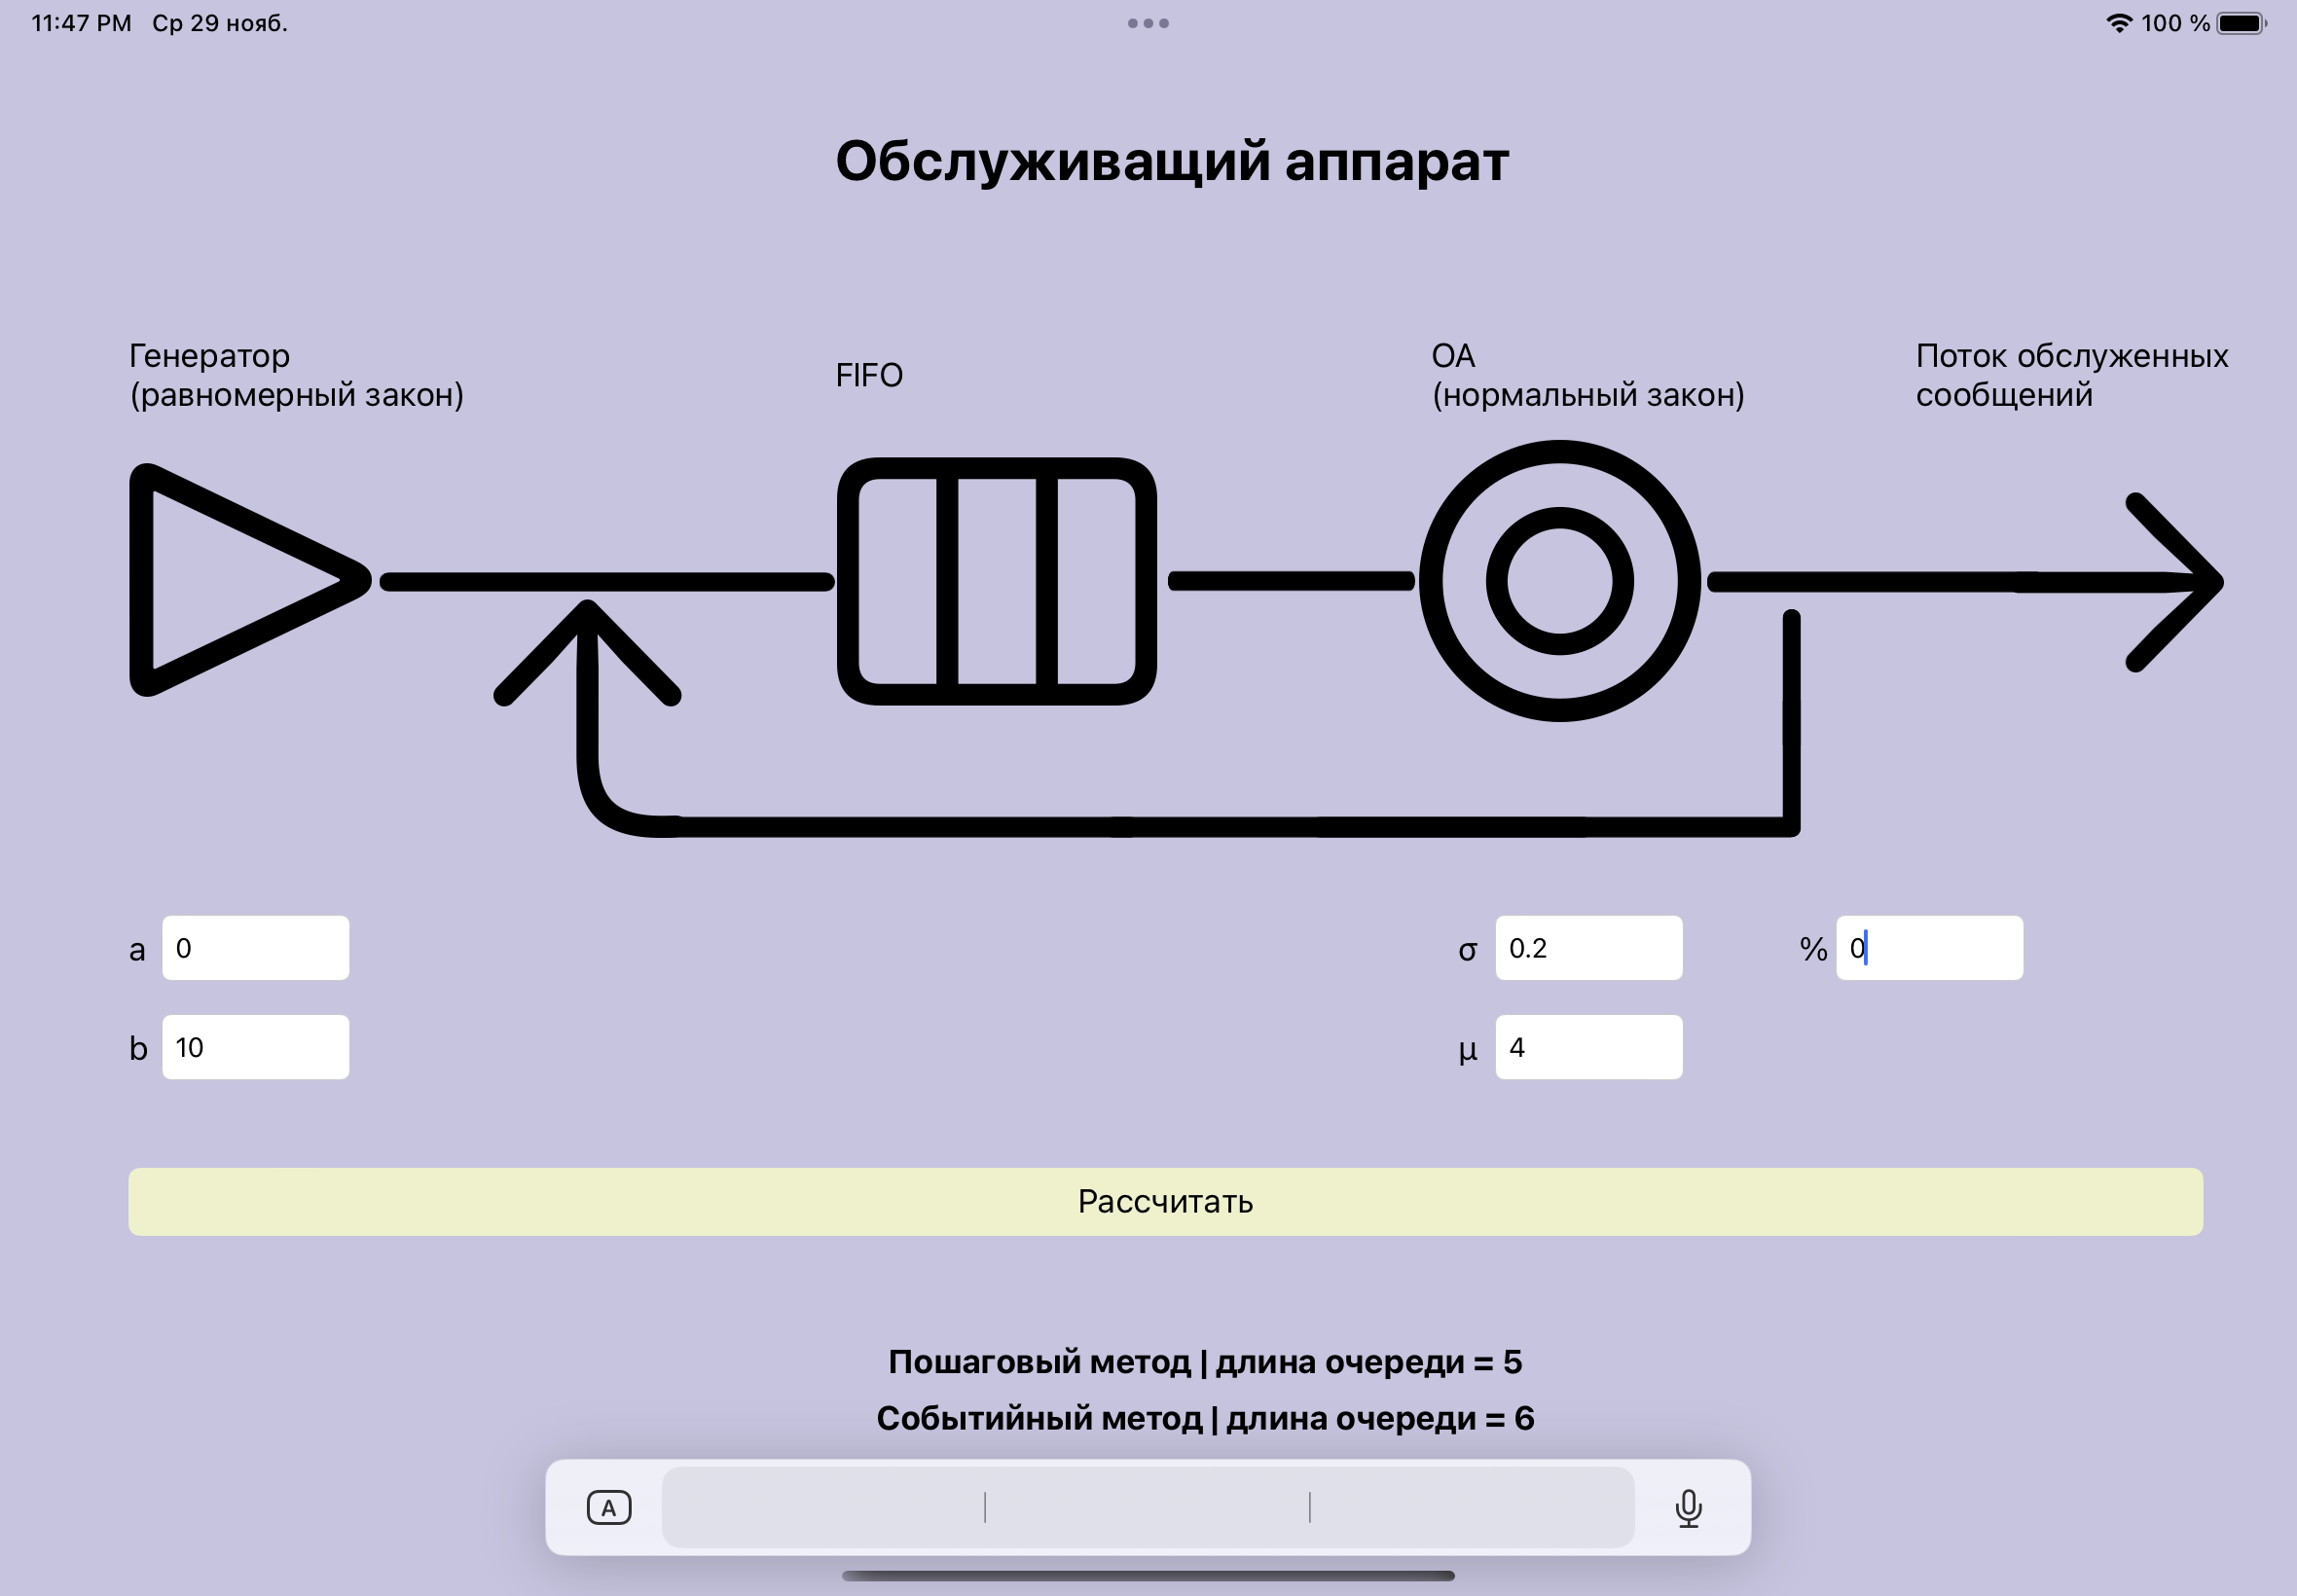
\includegraphics[scale = 0.15]{img/ex3.png}}
		\caption{Пример 3. Автомат обрабатывает сообщения интенсивнее, чем их создаёт генератор}
		\label{fig3:image}
	\end{center}
\end{figure}
\newpage

\begin{figure}[h!]
	\begin{center}
		{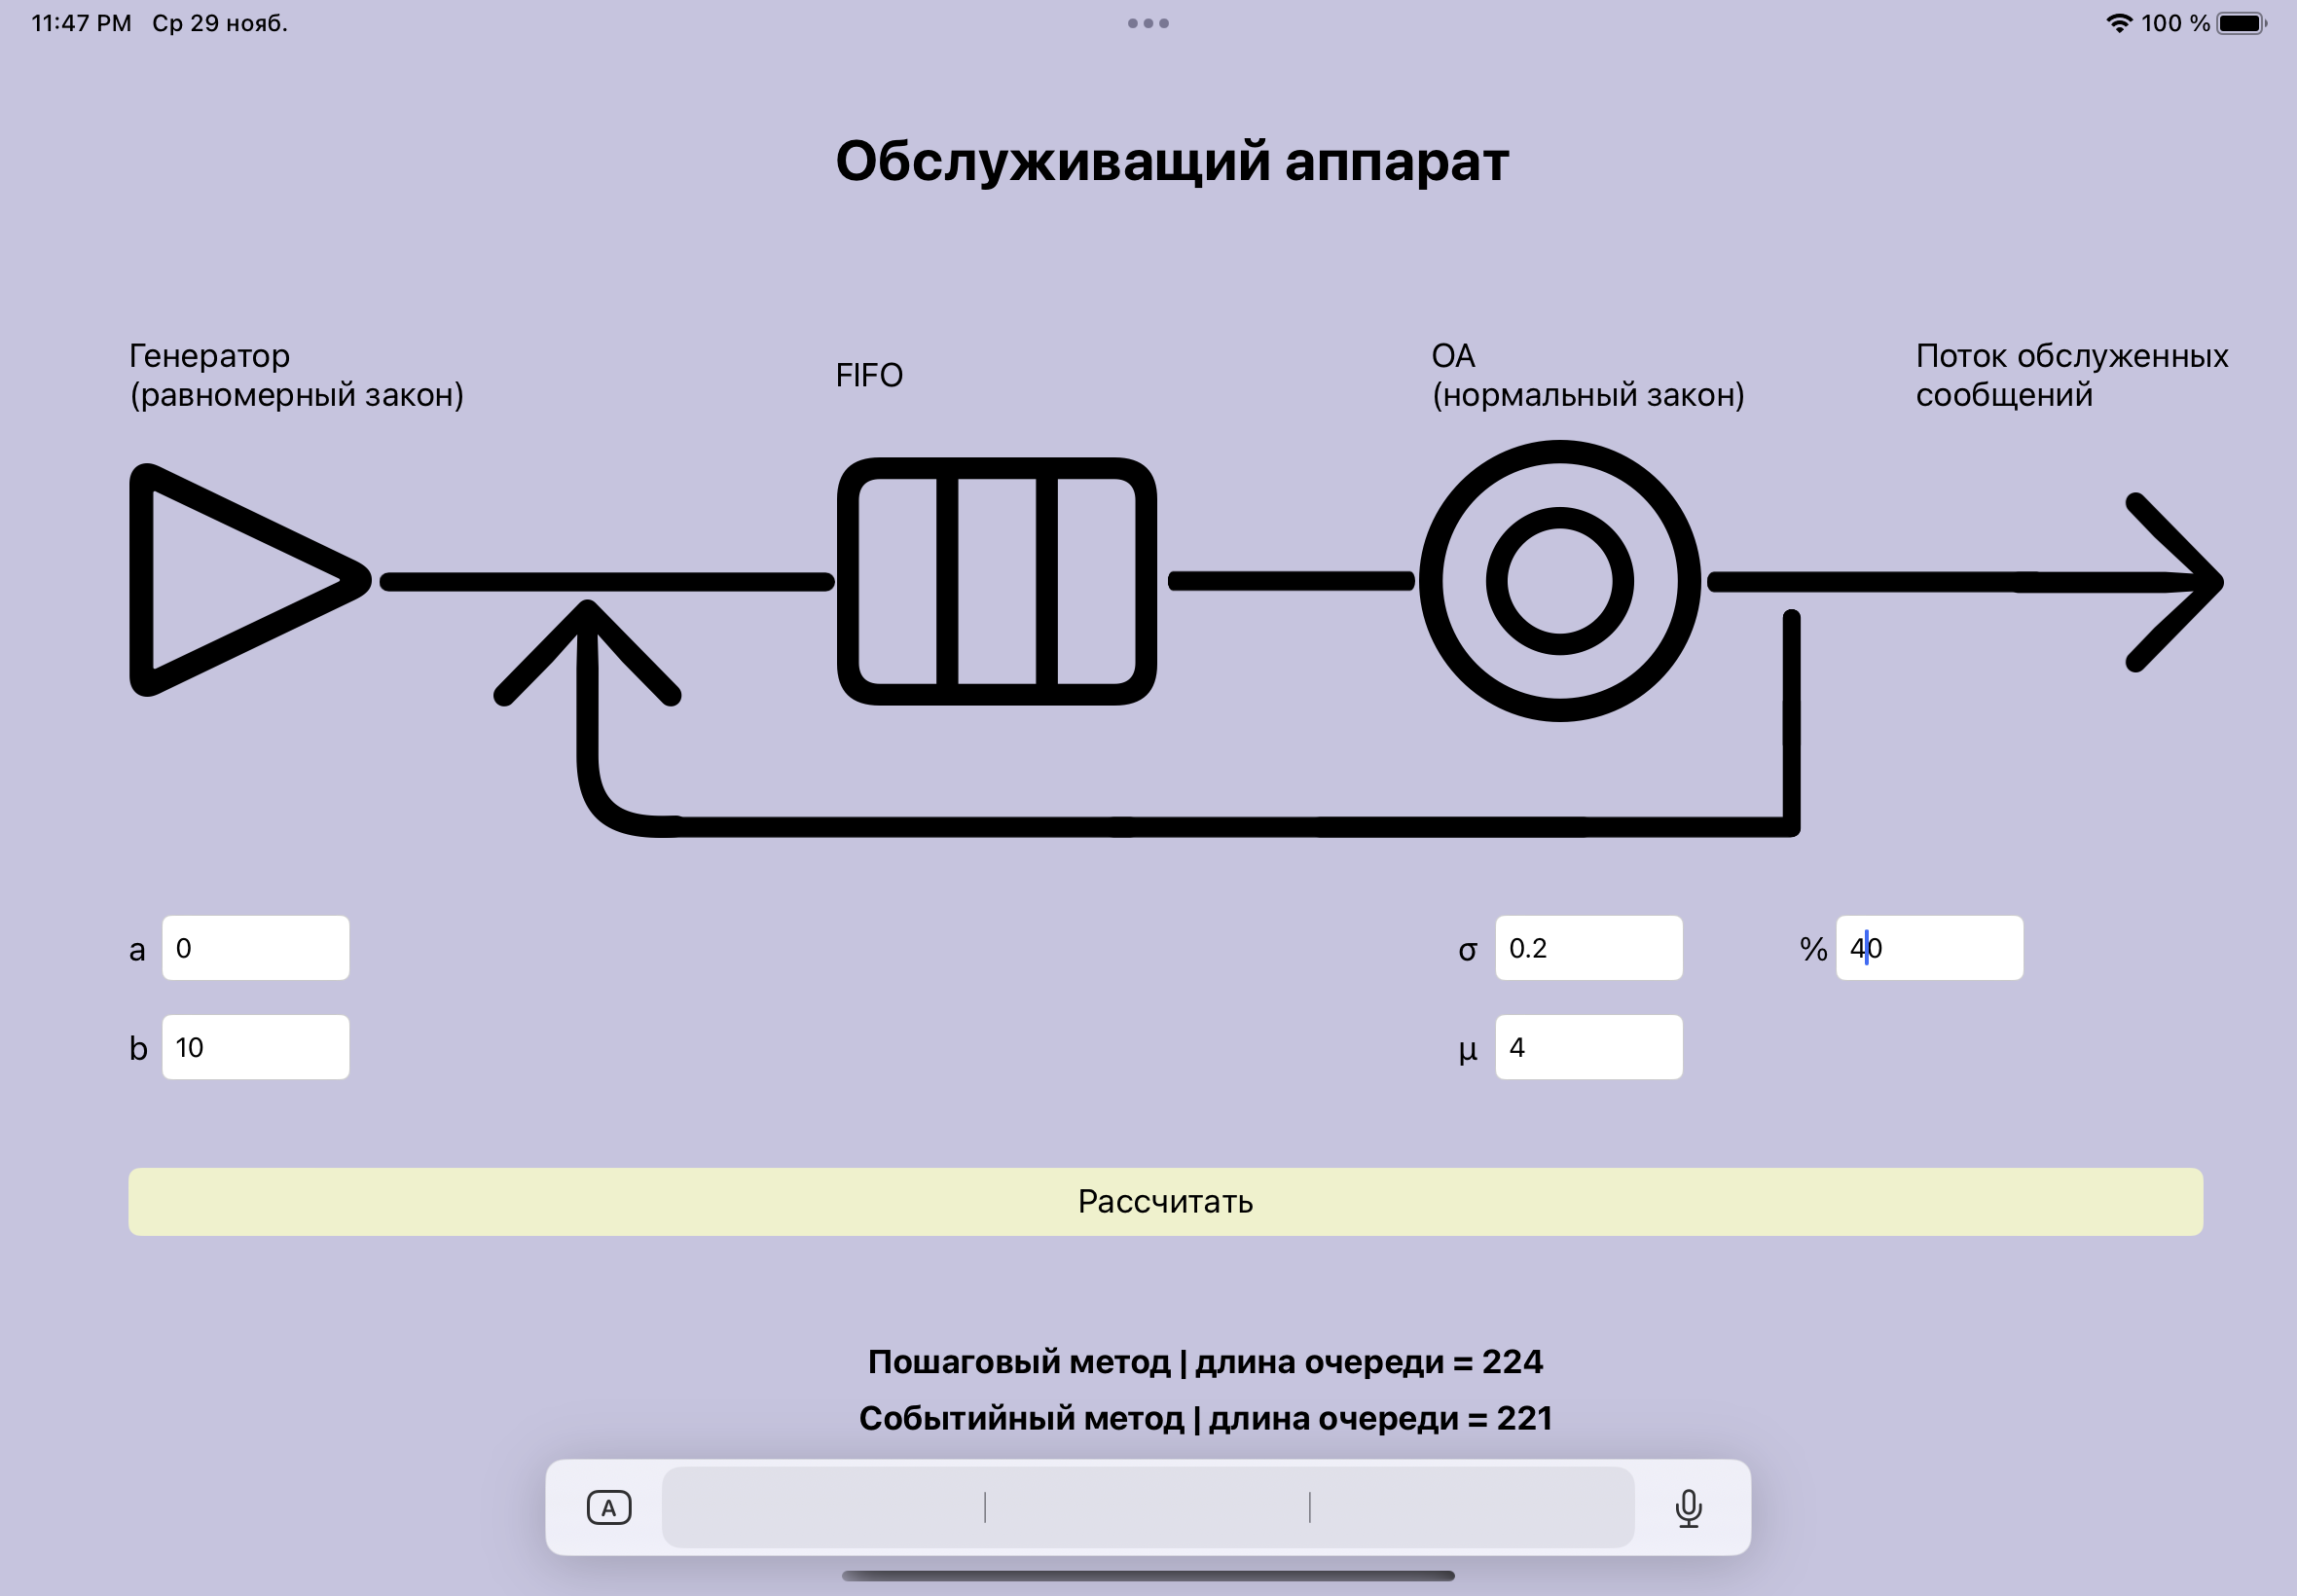
\includegraphics[scale = 0.15]{img/ex4.png}}
		\caption{Пример 4. Параметры такие же, как в примере 3, но есть процент возврата -- 40\%}
		\label{fig4:image}
	\end{center}
\end{figure}

\begin{figure}[h!]
	\begin{center}
		{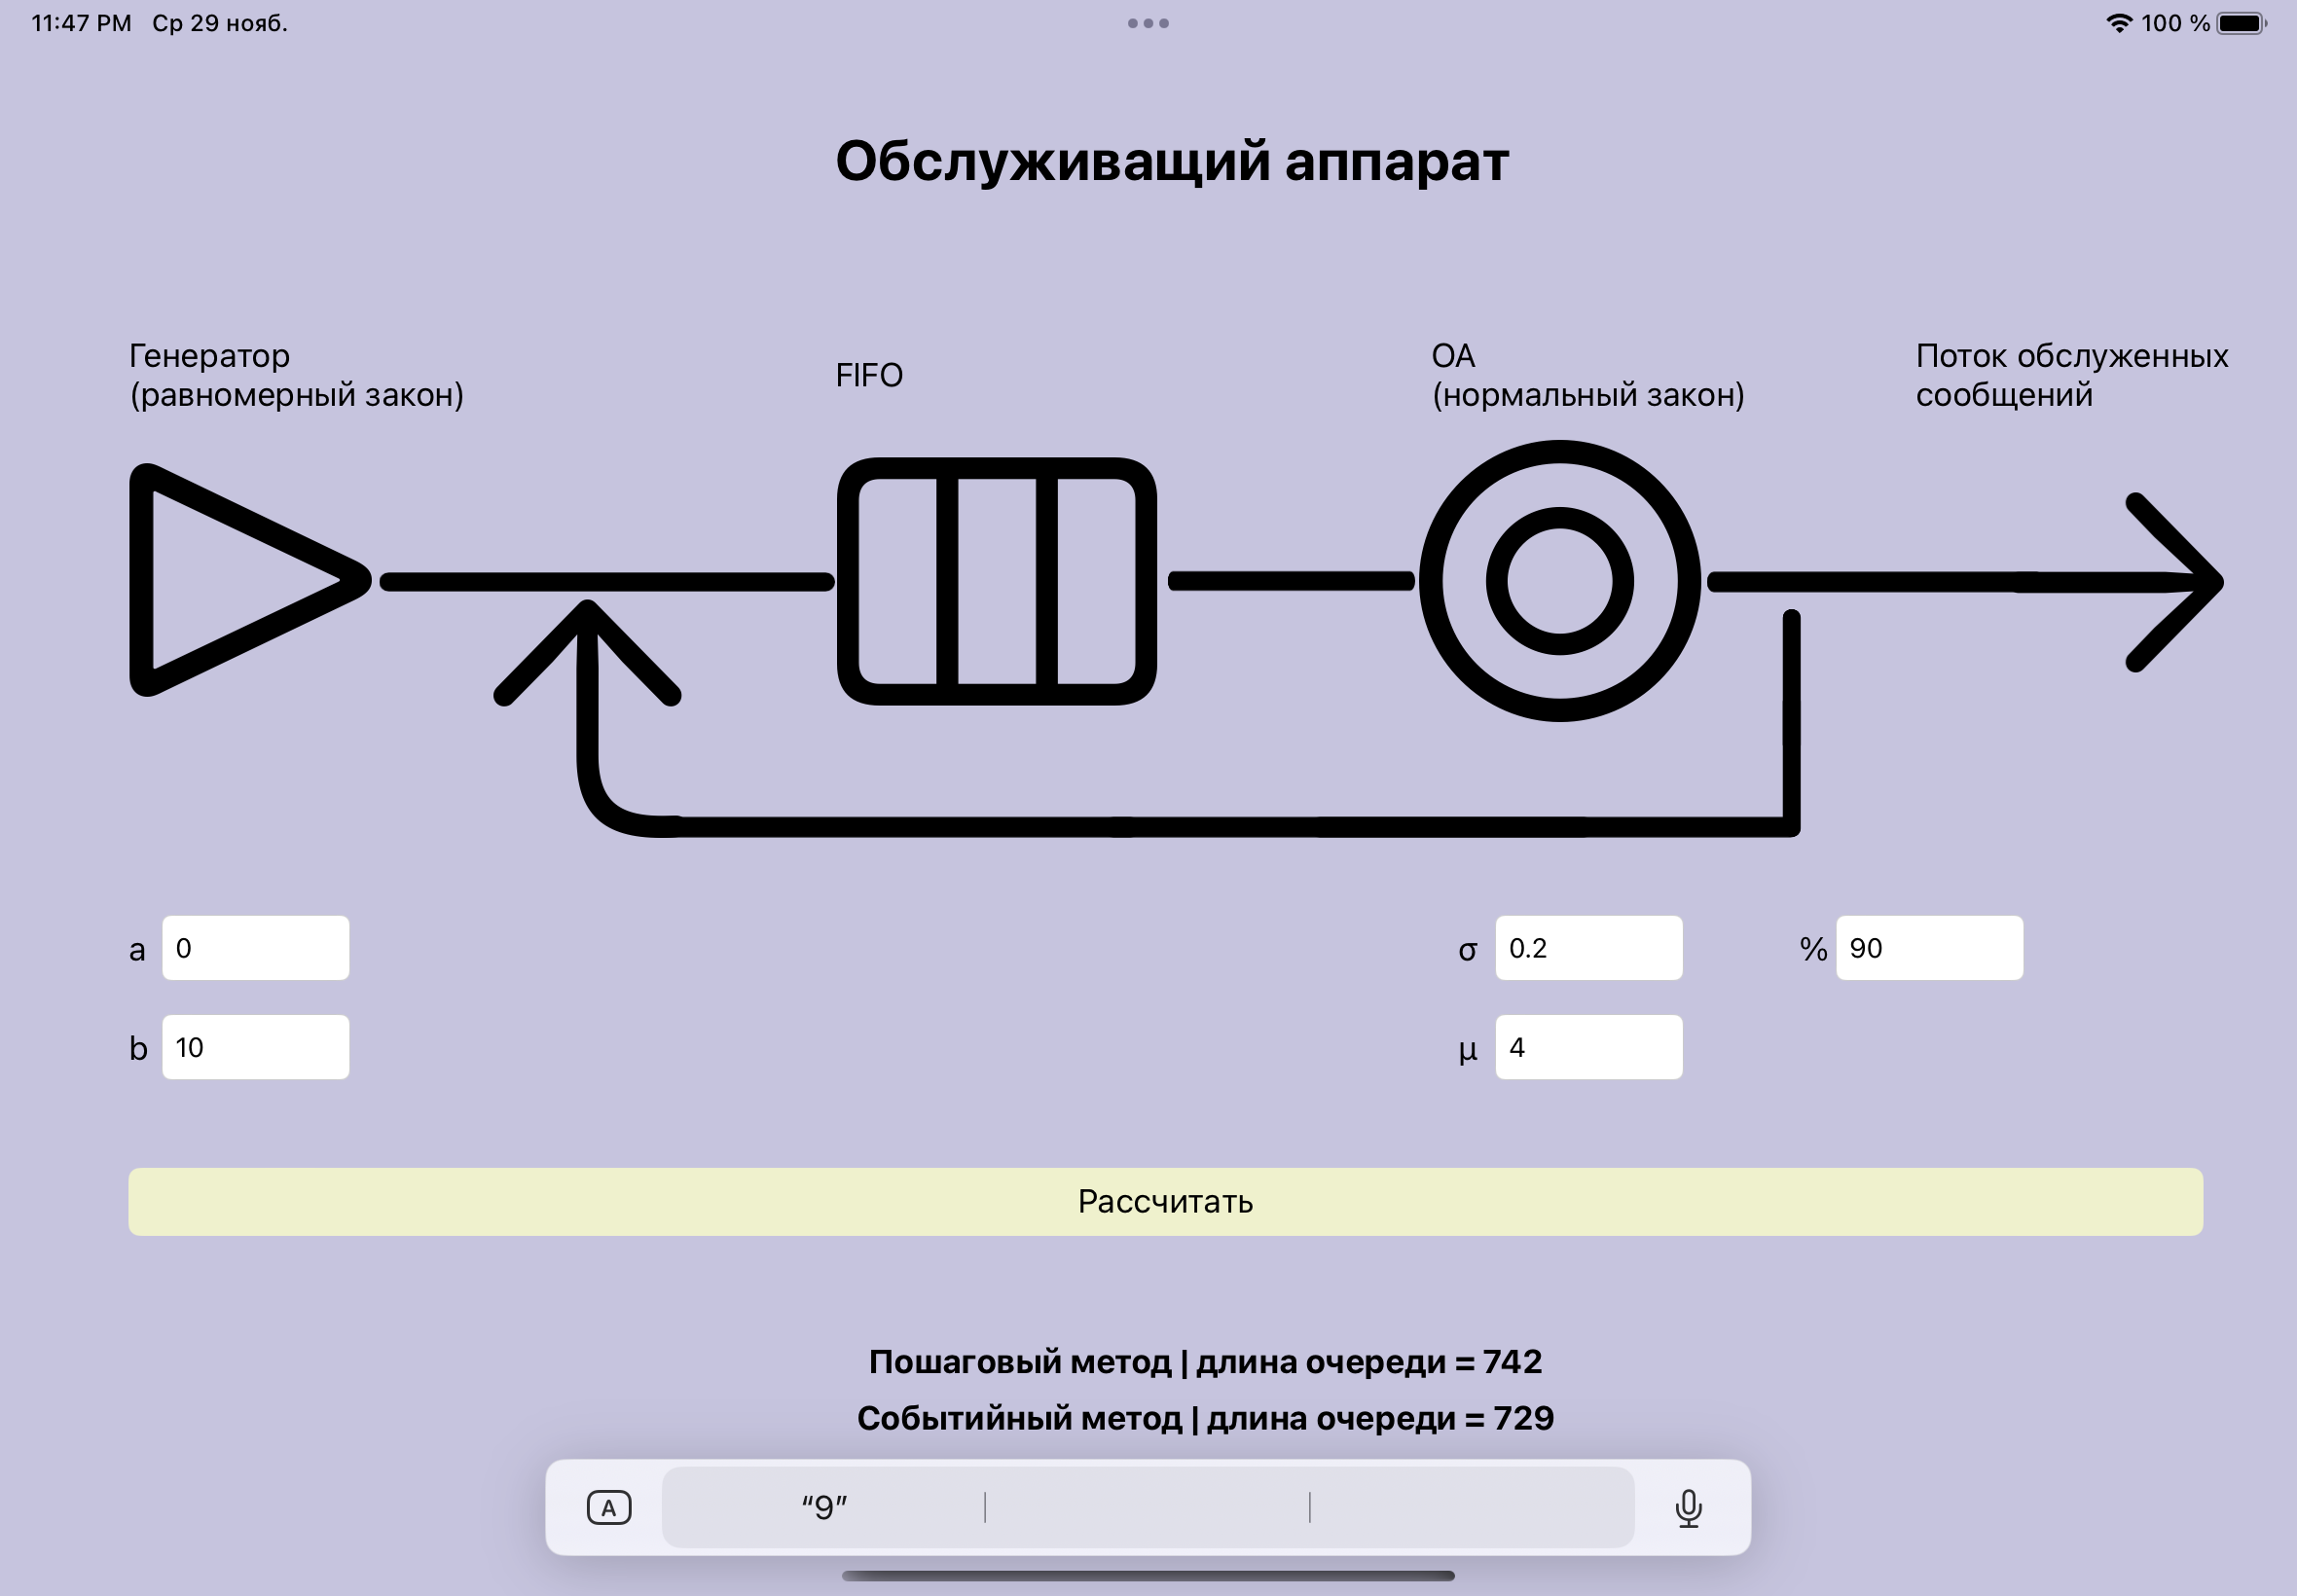
\includegraphics[scale = 0.15]{img/ex5.png}}
		\caption{Пример 5. Генератор и обслуживающий автомат работают с примерно одинаковой производительностью, но есть процент возврата  -- 90\%}
		\label{fig5:image}
	\end{center}
\end{figure}

\newpage


	\newpage
	

	
\end{document}
